\projecthead{06 / Robotics}{MIT Make - Harvard}{Mobile rover \& turret prototype}{Hackathon project}
\textit{Team prototype}
\par\medskip A wheeled rover carrying a small aiming turret, combining a camera-based recognition system with a compact mechanical assembly.
\par\smallskip {\small\color{muted} Tools: Mechanical integration, camera vision, 3D printing}
\medskip
\noindent
\begin{minipage}[t]{.48\linewidth}\centering\vspace{0pt}
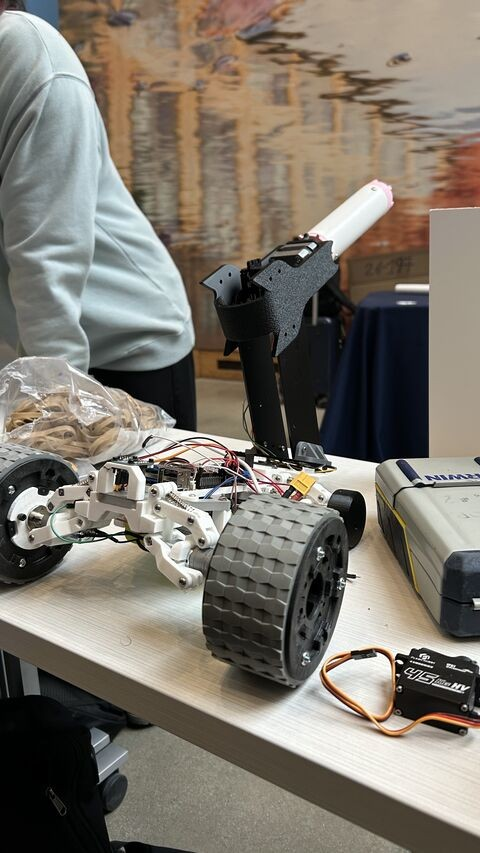
\includegraphics[width=\linewidth,height=1.8in,keepaspectratio]{images/mit-make/prototype.jpg}
\par\smallskip{\footnotesize\color{muted} Rover and turret on the bench.}\end{minipage}\hfill
\par\medskip
\subsection*{The prototype}
The robot combines a wheeled base, a small turret, and a launcher for short 3D-printed cylinders. Camera-based face recognition triggers the prototype behavior.
\subsection*{Mechanical integration}
The mechanical task was to package the launcher, aiming hardware, and wiring on a rover that could still move. The photograph documents the bench prototype.